%!TEX root = ../report.tex

\section{Frameworks for Client Authentication}
When having to authenticate users, we assume the scenario that we have a server $S1$ that the client $A$ wants to communicate with and additionally an authentication server $AS$ that is used to authenticate the client for $S1$.
There are different ways how these parties can communicate for this.
\begin{itemize}
  \item $S1$ uses the credentials provided by $A$ to run a cryptographic protocol with $AS$.
  \item End-to-end authentication between $A$ and $AS$. $S1$ relays messages and $AS$ informs $S1$ about the outcome (e.g.\ EAP).
  \item $A$ runs protocol with $AS$, interaction results in information $A$ and $S1$ can use to mutually authenticate (e.g.\ OAuth, Kerberos (original idea)).
\end{itemize}

\subsection{Kerberos}
Kerberos is an authentication and access control protocol service for work-station clusters which was developed with security, reliability, transparency and scalability as goals in mind.
\begin{figure}[H]
\centering
\hspace{50pt}
\begin{subfigure}{.6\textwidth}
  \centering
  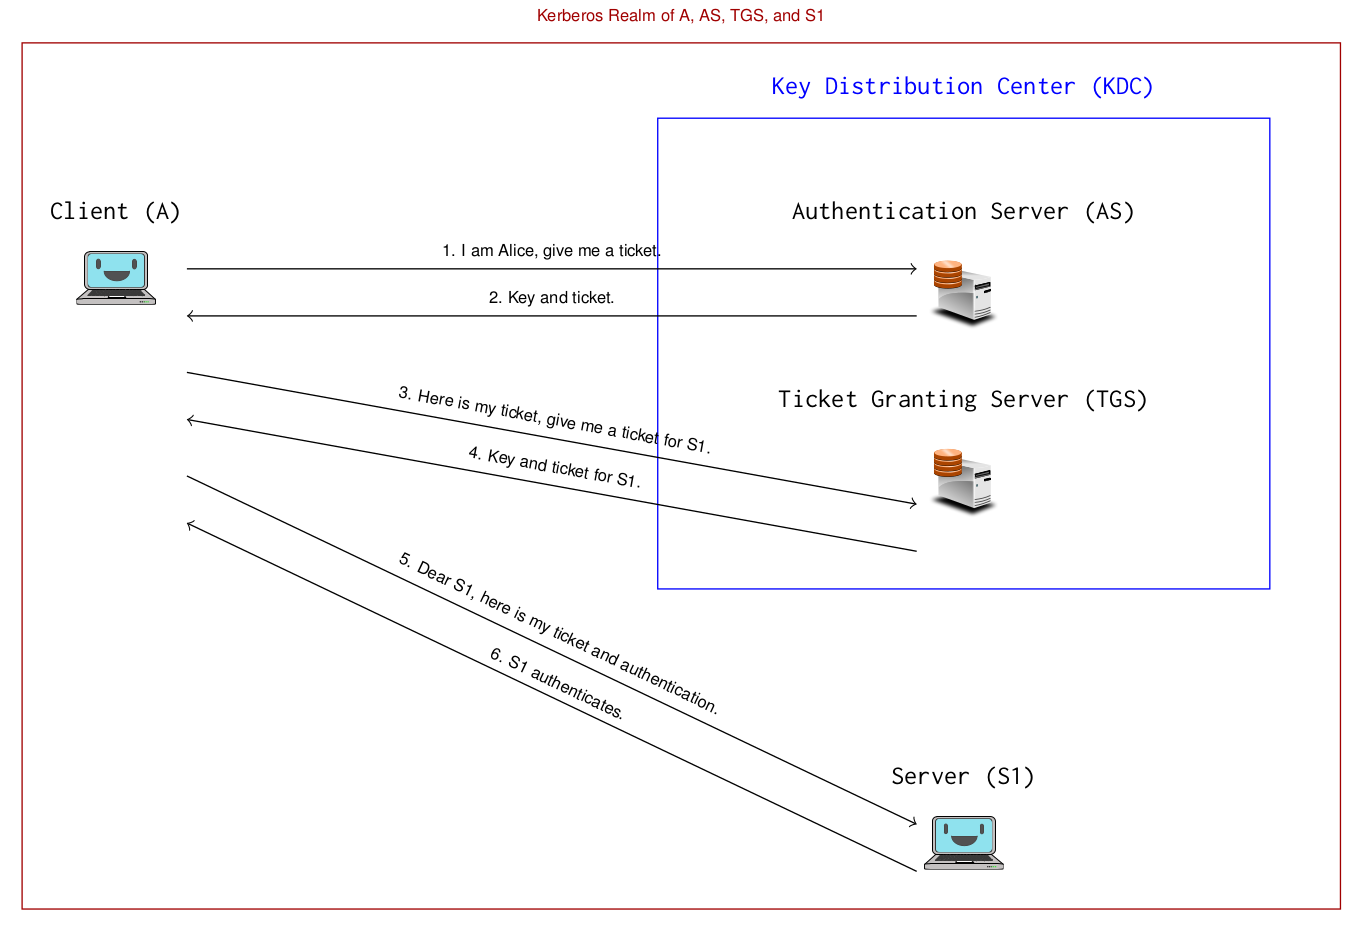
\includegraphics[width=\textwidth]{figures/kerberos_concept.png}
\end{subfigure}%
\newline
\begin{subfigure}{.6\textwidth}
  \centering
  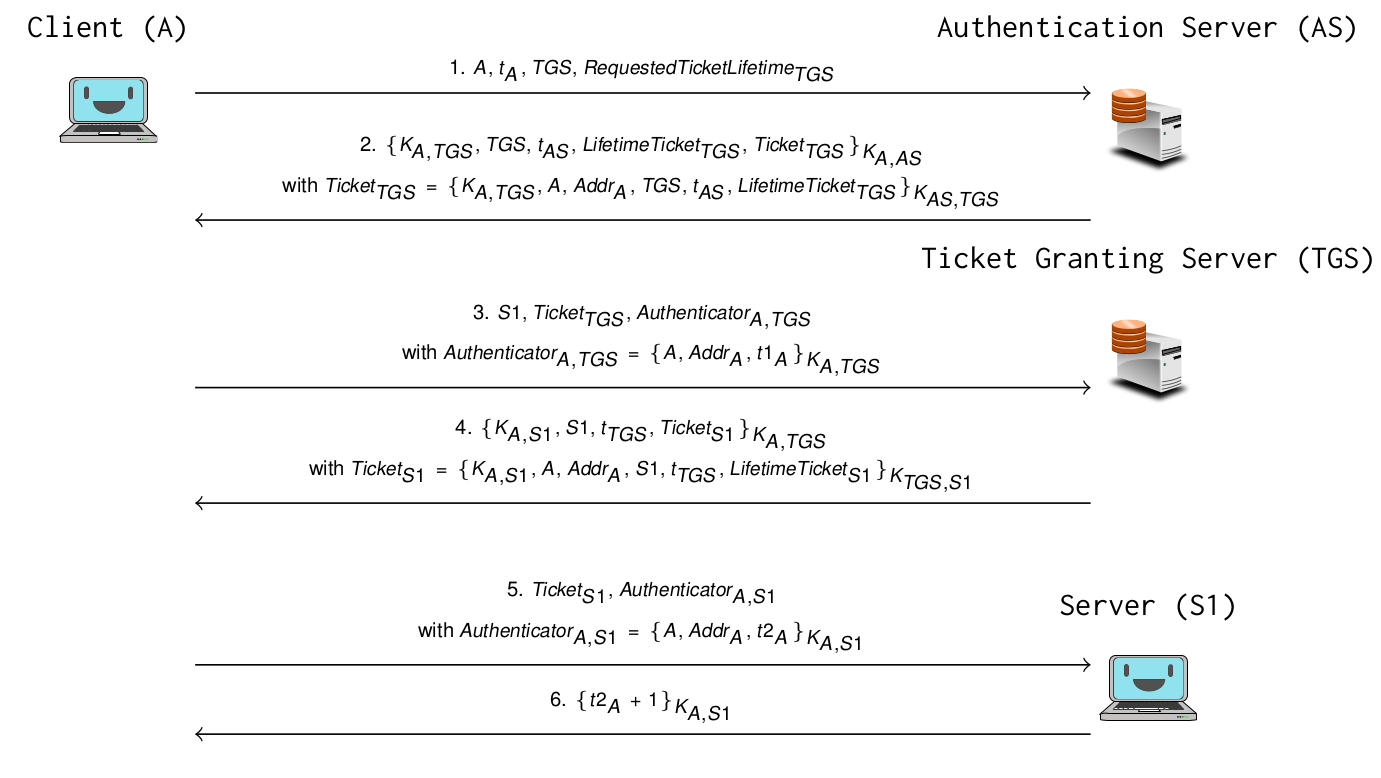
\includegraphics[width=\textwidth]{figures/kerberos_details.png}
\end{subfigure}
\caption{Kerberos}\label{fig:kerberos}
\end{figure}
AS and TGS are split into two separate parts to separate the concerns of authentication (AS) and authorization (TGS).
Before the protocol runs, $A$ and $AS$ have to know each other and have a long-term shared key $k_{AS,A} = h(Password_A)$ where $h$ is a hash function, usually md5.

\begin{figure}[H]
  \centering
  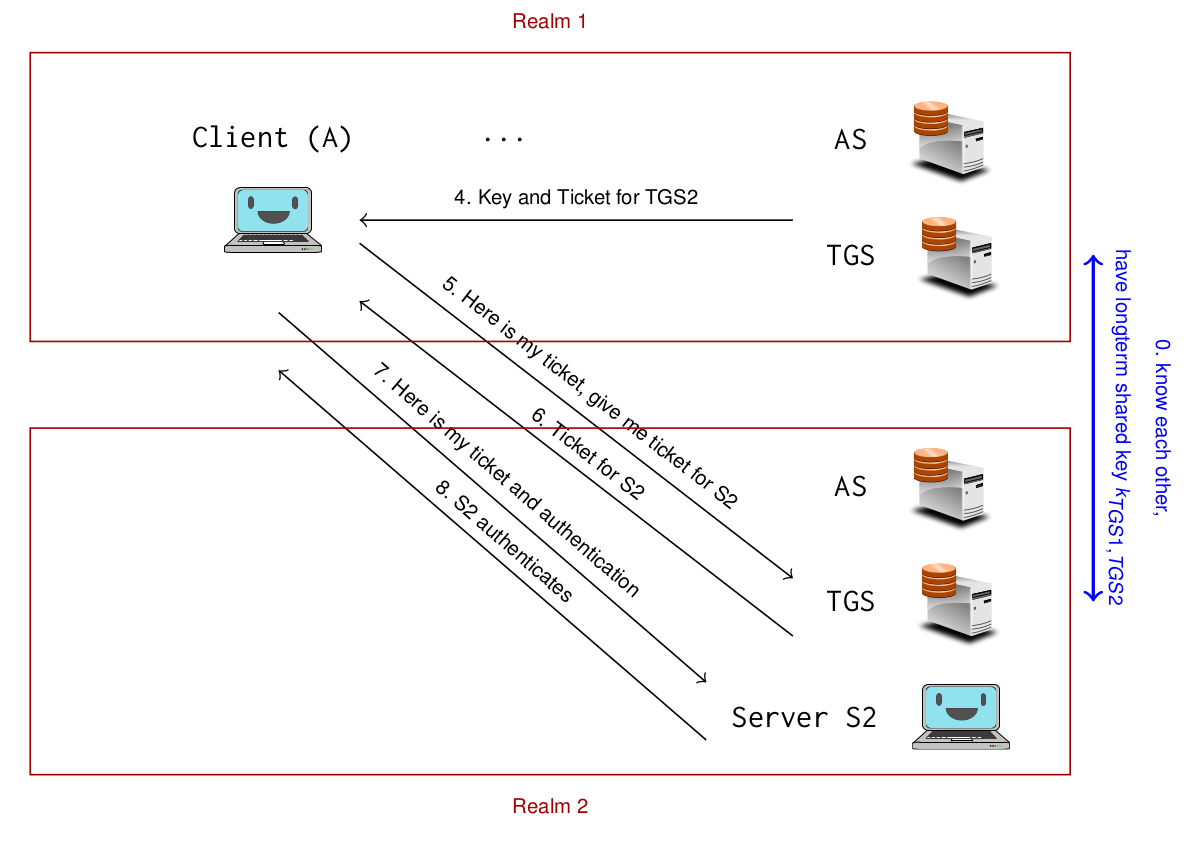
\includegraphics[width=.8\textwidth]{figures/kerberos_multi_realm.png}
  \caption{Kerberos Multi-Realm}\label{fig:kerberos_multi_realm}
\end{figure}
Keberos can also be used with multiple realms as shown in Figure~\ref{fig:kerberos_multi_realm}.\\

The biggest weakness of Kerberos is that message 1 is not protected and thus an attacker can request a ticket for someone else.
Since the second message is only encrypted with a password hash that often has low entropy, suitable attacks on the key can be performed like dictionary attacks.
To solve this, Kerberos pre-authentication can be used where communication partners first have to prove their identity before messages are further processed.
One of those methods is PA-ENC-TIMESTAMP in which $\{t_A\}_{K_{A,AS}}$ is added to message 1 as pre-authentication (not effective with an Dolev-Yao attacker model).
